% !TEX spellcheck = en_US



% ~~~~~~~~~~~~~~~~~~~~~~~~~~~~~~~~~~~~~~~ V
% (NC) 2026 Haluk Bingol
% github.com/halukbingol/LaTeX-Templates
%
% Licensees may copy, distribute, display, and perform the work and make derivative works 
% and remixes based on it only for non-commercial purposes. 
% ~~~~~~~~~~~~~~~~~~~~~~~~~~~~~~~~~~~~~~~ A




% =====================================================================
%  The Eclipse IDE -- Concepts: Workspace, Workbench, Build, Run and Debug
%  ---------------------------------------------------------------------
%  Built on hblib/Template/hblibTemplate.tex with the libraries in ../../hblib/.
%  Programs and their real outputs are in codeoutput/:
%     codeoutput/<Name>.java  a program (classes without main() are only compiled)
%     codeoutput/<Name>.sh    a terminal session, run in a copy of codeoutput/<Name>/
%     codeoutput/<Name>.txt   what it printed, made by:  bash run_examples.sh
% =====================================================================

\documentclass[aspectratio=169,10pt,compress]{beamer}

% ~~~~~~~~~~~~~~~~~~~~~~~~~~~~~~~~~~~~~~~~~~~~~~~~~~~~~~~~~~~~~~~~~ V hblib
	\usepackage{../../hblib/hblibPresentation} % lib presentation: theme, i/N, \hSection, algorithm2e, ...
	\usepackage{../../hblib/hblibCodeoutput} % lib code + output: \lstcode, \lstterminal, ...
	\usepackage{../../hblib/hblibDatastructures} % lib data structures: \hString, \hStack, \hQueue
% ~~~~~~~~~~~~~~~~~~~~~~~~~~~~~~~~~~~~~~~~~~~~~~~~~~~~~~~~~~~~~~~~~ A hblib


% theme, i/N, fonts (T1, lmodern), booktabs, xcolor, array (L{width} columns), listings, tikz,
% algorithm2e (\small captions, \Fn) and the color gitred come from the hblib libraries




% +++++++++++++++++++++++++++++++++++++++ V specific
\DontPrintSemicolon % in algorithms
\newcommand{\win}{\textbf{Windows}}
\newcommand{\mac}{\textbf{macOS}}
% +++++++++++++++++++++++++++++++++++++++ A specific

% ---------------------------------------------------------------------
\title{The Eclipse IDE}
\subtitle{Concepts: Workspace, Workbench, Build, Run and Debug}
\author[Bingol]{Haluk O. Bingol}

\institute[FCIS]{
    Faculty of Computer and Information Sciences\\
    Yeditepe University
}
\date{
	{\tiny \hbTimeStamp}
}

\begin{document}




% ~~~~~~~~~~~~~~~~~~~~~~~~~~~~~~~~~~~~~~ V frm
\begin{frame}[t,fragile]
  \titlepage
\end{frame}
% ~~~~~~~~~~~~~~~~~~~~~~~~~~~~~~~~~~~~~~ A frm




% ~~~~~~~~~~~~~~~~~~~~~~~~~~~~~~~~~~~~~~ V frm
\begin{frame}[t,fragile] \frametitle{Outline}
  \begin{columns}[T]
    \begin{column}{0.48\textwidth}
      \tableofcontents[sections={1-4}, hideallsubsections]
    \end{column}
    \begin{column}{0.48\textwidth}
      \tableofcontents[sections={5-8}, hideallsubsections]
    \end{column}
  \end{columns}
\end{frame}
% ~~~~~~~~~~~~~~~~~~~~~~~~~~~~~~~~~~~~~~ A frm

% ~~~~~~~~~~~~~~~~~~~~~~~~~~~~~~~~~~~~~~ V
\hSection[IDE]{What Is an IDE?}
% ~~~~~~~~~~~~~~~~~~~~~~~~~~~~~~~~~~~~~~ A




% ~~~~~~~~~~~~~~~~~~~~~~~~~~~~~~~~~~~~~~ V frm
\begin{frame}[t,fragile] \frametitle{From separate tools to one window}
  \begin{center}
  \begin{tikzpicture}[tool/.style={draw, thick, rounded corners, minimum width=2.2cm, minimum height=0.8cm, font=\small, align=center}]
    \node[tool, fill=yellow!20] (e) at (0,0)   {editor};
    \node[tool, fill=green!15]  (c) at (3,0)   {compiler\\ \scriptsize\texttt{javac}};
    \node[tool, fill=blue!12]   (r) at (6,0)   {runner\\ \scriptsize\texttt{java}};
    \node[tool, fill=red!12]    (g) at (9,0)   {debugger\\ \scriptsize\texttt{jdb}};
    \node[tool, fill=gray!15]   (v) at (12,0)  {version control\\ \scriptsize\texttt{git}};
    \draw[very thick, rounded corners, colorGo] (-1.4,-0.8) rectangle (13.4,0.8);
    \node[font=\small\bfseries, colorGo] at (6,-1.15) {Integrated Development Environment: one window, one project model};
  \end{tikzpicture}
  \end{center}
  \begin{itemize}\small
    \item The IDE \textbf{understands} the program: it knows every class, method and variable while you type.
    \item So it can \textbf{complete} code, \textbf{mark} errors at once, \textbf{rename} safely in all files and \textbf{stop} a running program at a line.
    \item The tools are the same as on the command line; the IDE connects them.
  \end{itemize}
\end{frame}
% ~~~~~~~~~~~~~~~~~~~~~~~~~~~~~~~~~~~~~~ A frm




% ~~~~~~~~~~~~~~~~~~~~~~~~~~~~~~~~~~~~~~ V frm
\begin{frame}[t,fragile] \frametitle{Eclipse in a nutshell}
  \begin{columns}[T]
    \begin{column}{0.5\textwidth}
      \begin{itemize}\small
        \item Started at IBM; open source since \textbf{2001}; run by the \textbf{Eclipse Foundation} since 2004.
        \item Free, license EPL-2.0; Windows, macOS, Linux.
        \item A new release every \textbf{three months}, named by date: \textbf{2026-06} is Eclipse 4.40.
        \item Download from \texttt{eclipse.org}: the \emph{Eclipse IDE for Java Developers} package
              includes the Java runtime that Eclipse itself needs.
      \end{itemize}
    \end{column}
    \begin{column}{0.46\textwidth}
      \begin{center}\small
      \begin{tabular}{ll}
        \toprule
        \textbf{IDE}            & \textbf{Java support from} \\
        \midrule
        Eclipse                 & JDT (Java Development Tools) \\
        VS Code                 & extension based on Eclipse JDT \\
        IntelliJ IDEA           & JetBrains, own engine \\
        NetBeans                & Apache, uses \texttt{javac} \\
        \bottomrule
      \end{tabular}
      \end{center}
      \small The skills move between IDEs: projects, build path, run, debug, refactor.
    \end{column}
  \end{columns}
\end{frame}
% ~~~~~~~~~~~~~~~~~~~~~~~~~~~~~~~~~~~~~~ A frm

% ~~~~~~~~~~~~~~~~~~~~~~~~~~~~~~~~~~~~~~ V
\hSection[Workspace]{Workspace and Projects}
% ~~~~~~~~~~~~~~~~~~~~~~~~~~~~~~~~~~~~~~ A




% ~~~~~~~~~~~~~~~~~~~~~~~~~~~~~~~~~~~~~~ V frm
\begin{frame}[t,fragile] \frametitle{Workspace, projects, files}
  \begin{columns}[T]
    \begin{column}{0.5\textwidth}
      \begin{center}
      \begin{tikzpicture}[htree, level distance=0.95cm, level 1/.style={sibling distance=2.2cm}, level 2/.style={sibling distance=1.0cm}, scale=0.8, transform shape]
  \node[hsquare] {workspace} child {node[hsquare] {.metadata}} child {node[hsquare, hdone] {Hello} child {node[hsquare] {src}} child {node[hsquare] {bin}}} child {node[hsquare, hdone] {Lab2}};
\end{tikzpicture}
      \end{center}
    \end{column}
    \begin{column}{0.46\textwidth}
      \begin{itemize}\small
        \item \textbf{Workspace}: a folder that holds your projects and Eclipse's settings (\texttt{.metadata}).
              Eclipse asks for it at start.
        \item \textbf{Project}: one program or library; Eclipse builds, runs and shares it as a unit.
        \item Java project: sources in \texttt{src/}, compiled classes in \texttt{bin/}.
        \item The project's settings are plain files: \texttt{.project}, \texttt{.classpath}, \texttt{.settings/}.
      \end{itemize}
    \end{column}
  \end{columns}
\end{frame}
% ~~~~~~~~~~~~~~~~~~~~~~~~~~~~~~~~~~~~~~ A frm




% ~~~~~~~~~~~~~~~~~~~~~~~~~~~~~~~~~~~~~~ V frm
\begin{frame}[t,fragile] \frametitle{The workbench window}
  \begin{columns}[T]
    \begin{column}{0.6\textwidth}
      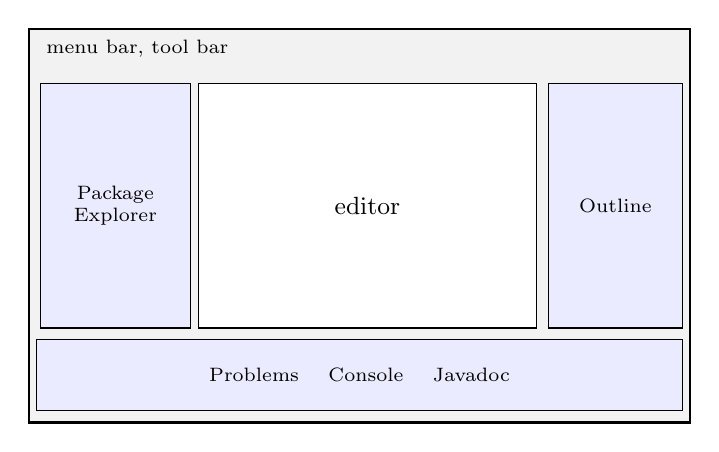
\begin{tikzpicture}[v/.style={draw, fill=blue!8, font=\scriptsize, align=center}, x=1cm, y=1cm]
        \draw[thick, fill=gray!10] (0,0) rectangle (8.4,5);
        \node[font=\scriptsize, anchor=west] at (0.1,4.75) {menu bar, tool bar};
        \node[v, minimum width=1.9cm, minimum height=3.1cm] at (1.1,2.75) {Package\\ Explorer};
        \node[draw, fill=white, font=\small, minimum width=4.3cm, minimum height=3.1cm] at (4.3,2.75) {editor};
        \node[v, minimum width=1.7cm, minimum height=3.1cm] at (7.45,2.75) {Outline};
        \node[v, minimum width=8.2cm, minimum height=0.9cm] at (4.2,0.6) {Problems \quad Console \quad Javadoc};
      \end{tikzpicture}
    \end{column}
    \begin{column}{0.36\textwidth}
      \begin{itemize}\small
        \item \textbf{Editors} (middle): files you change; a \texttt{*} in the tab means unsaved.
        \item \textbf{Views} (around): information about the project: files, problems, output.
        \item A \textbf{perspective} is an arrangement of views for one job.
      \end{itemize}
    \end{column}
  \end{columns}
\end{frame}
% ~~~~~~~~~~~~~~~~~~~~~~~~~~~~~~~~~~~~~~ A frm




% ~~~~~~~~~~~~~~~~~~~~~~~~~~~~~~~~~~~~~~ V frm
\begin{frame}[t,fragile] \frametitle{Perspectives}
  \begin{center}\small
  \begin{tabular}{lll}
    \toprule
    \textbf{perspective} & \textbf{for}               & \textbf{main views} \\
    \midrule
    Java                 & writing code               & Package Explorer, Outline, Problems, Console \\
    Debug                & a stopped program          & Debug (threads, stack), Variables, Breakpoints, Expressions \\
    Git                  & version control            & Git Repositories, Git Staging, History \\
    \bottomrule
  \end{tabular}
  \end{center}
  \begin{itemize}\small
    \item Switch with the buttons at the top right, or \menu{Window > Perspective > Open Perspective}.
    \item Lost a view or messed up the layout? \menu{Window > Perspective > Reset Perspective}.
    \item Any view: \menu{Window > Show View}.
  \end{itemize}
\end{frame}
% ~~~~~~~~~~~~~~~~~~~~~~~~~~~~~~~~~~~~~~ A frm

% ~~~~~~~~~~~~~~~~~~~~~~~~~~~~~~~~~~~~~~ V
\hSection[Build]{Building: the Eclipse Compiler}
% ~~~~~~~~~~~~~~~~~~~~~~~~~~~~~~~~~~~~~~ A




% ~~~~~~~~~~~~~~~~~~~~~~~~~~~~~~~~~~~~~~ V frm
\begin{frame}[t,fragile] \frametitle{Build automatically}
  \begin{center}
  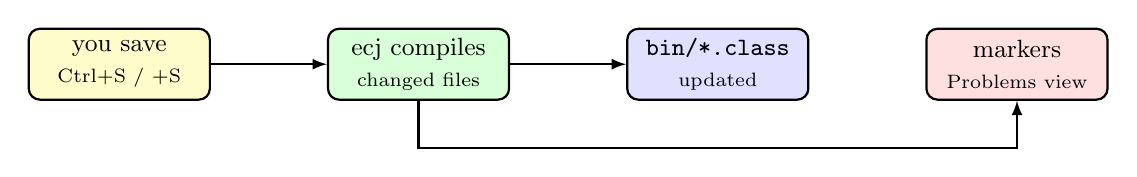
\begin{tikzpicture}[st/.style={draw, thick, rounded corners, minimum width=2.3cm, minimum height=0.9cm, align=center, font=\small}]
    \node[st, fill=yellow!20] (s) at (0,0)    {you save\\ \scriptsize\keys{Ctrl+S} / \keys{\cmd+S}};
    \node[st, fill=green!15]  (c) at (3.8,0)  {ecj compiles\\ \scriptsize changed files};
    \node[st, fill=blue!12]   (b) at (7.6,0)  {\texttt{bin/*.class}\\ \scriptsize updated};
    \node[st, fill=red!12]    (p) at (11.4,0) {markers\\ \scriptsize Problems view};
    \draw[-latex, thick] (s) -- (c);  \draw[-latex, thick] (c) -- (b);  \draw[-latex, thick] (c.south) |- ++(0,-0.6) -| (p.south);
  \end{tikzpicture}
  \end{center}
  \begin{itemize}\small
    \item Eclipse has its \textbf{own Java compiler}, \texttt{ecj}, not \texttt{javac}. It compiles \textbf{on every save}
          (\menu{Project > Build Automatically}).
    \item Errors and warnings become \textbf{markers}: red/yellow icons in the editor and lines in the \textbf{Problems} view.
    \item No separate ``compile'' step: when the Problems view is empty, the program is ready to run.
  \end{itemize}
\end{frame}
% ~~~~~~~~~~~~~~~~~~~~~~~~~~~~~~~~~~~~~~ A frm




% ~~~~~~~~~~~~~~~~~~~~~~~~~~~~~~~~~~~~~~ V frm
\begin{frame}[t,fragile] \frametitle{The same messages from the command line}
  \lstterminal[basicstyle=\ttfamily\scriptsize]{codeoutput/Problems.txt}

  \vspace{0.1em}
  \small
  This is \texttt{ecj}, the compiler inside Eclipse, run in a terminal: the Problems view shows exactly these messages,
  one per line, and the editor underlines the \texttt{\textasciicircum} positions.
\end{frame}
% ~~~~~~~~~~~~~~~~~~~~~~~~~~~~~~~~~~~~~~ A frm




% ~~~~~~~~~~~~~~~~~~~~~~~~~~~~~~~~~~~~~~ V frm
\begin{frame}[t,fragile] \frametitle{Incremental build}
  \begin{columns}[T]
    \begin{column}{0.55\textwidth}
      \SetAlFnt{\small}


% +++++++++++++++++++++++++++++++++++++++ V alg
%: -Alg. 
\begin{algorithm}[H]
  \caption{Build after a save}
  \KwIn{the files changed since the last build}
  \ForEach{changed file $f$}{
    compile $f$; replace the markers of $f$\;
    \If{the public shape of a type in $f$ changed}{
      add every file that uses that type to the work list\;
    }
  }
  compile the work list the same way, until it is empty\;
\end{algorithm}
% +++++++++++++++++++++++++++++++++++++++ A alg

    \end{column}
    \begin{column}{0.41\textwidth}
      \begin{itemize}\small
        \item Only what changed is compiled: fast even for big projects.
        \item ``Public shape'': method signatures, fields, class names. Changing a method body does not affect other files.
        \item If things look wrong: \menu{Project > Clean\dots} rebuilds everything.
      \end{itemize}
    \end{column}
  \end{columns}
\end{frame}
% ~~~~~~~~~~~~~~~~~~~~~~~~~~~~~~~~~~~~~~ A frm

% ~~~~~~~~~~~~~~~~~~~~~~~~~~~~~~~~~~~~~~ V
\hSection[Run]{Running Programs}
% ~~~~~~~~~~~~~~~~~~~~~~~~~~~~~~~~~~~~~~ A




% ~~~~~~~~~~~~~~~~~~~~~~~~~~~~~~~~~~~~~~ V frm
\begin{frame}[t,fragile] \frametitle{Run and launch configurations}
  \begin{columns}[T]
    \begin{column}{0.5\textwidth}
      \begin{itemize}\small
        \item \menu{Run As > Java Application} (right click on a class with \texttt{main}) runs it; output and keyboard input
              go through the \textbf{Console} view.
        \item The first run creates a \textbf{launch configuration}: which class, which JRE,
              \textbf{program arguments} (\texttt{args}), \textbf{VM arguments} (e.g.\ \texttt{-ea}).
        \item Edit them in \menu{Run > Run Configurations\dots}
      \end{itemize}
    \end{column}
    \begin{column}{0.46\textwidth}
      \begin{center}\footnotesize
      \begin{tabular}{@{}lll@{}}
        \toprule
        \textbf{task}   & \win              & \mac \\
        \midrule
        run again       & \keys{Ctrl+F11}   & \keys{\cmd+\shift+F11} \\
        debug again     & \keys{F11}        & \keys{\cmd+F11} \\
        stop            & \multicolumn{2}{l}{red square in the Console} \\
        \bottomrule
      \end{tabular}
      \end{center}
      \small Laptop keyboards may need \keys{Fn} for the F keys.
    \end{column}
  \end{columns}
\end{frame}
% ~~~~~~~~~~~~~~~~~~~~~~~~~~~~~~~~~~~~~~ A frm

% ~~~~~~~~~~~~~~~~~~~~~~~~~~~~~~~~~~~~~~ V
\hSection[Debug]{Debugging}
% ~~~~~~~~~~~~~~~~~~~~~~~~~~~~~~~~~~~~~~ A




% ~~~~~~~~~~~~~~~~~~~~~~~~~~~~~~~~~~~~~~ V frm
\begin{frame}[t,fragile] \frametitle{Stop the program and look inside}
  \begin{columns}[T]
    \begin{column}{0.5\textwidth}
      \begin{itemize}\small
        \item \textbf{Breakpoint}: double-click the left margin of a line (a blue dot).
        \item \textbf{Debug As > Java Application}: the program runs until it reaches a breakpoint, then
              Eclipse switches to the \textbf{Debug perspective}.
        \item \textbf{Variables} view: the current values; change them, too.
        \item \textbf{Expressions} view: any expression, e.g.\ \texttt{sum / 3.0}.
      \end{itemize}
    \end{column}
    \begin{column}{0.46\textwidth}
      \begin{center}\footnotesize
      \begin{tabular}{@{}lll@{}}
        \toprule
        \textbf{step}       & \textbf{key} & \textbf{meaning} \\
        \midrule
        Step Into           & \keys{F5}    & go into the called method \\
        Step Over           & \keys{F6}    & run the line, stop at the next \\
        Step Return         & \keys{F7}    & finish this method \\
        Resume              & \keys{F8}    & run to the next breakpoint \\
        \bottomrule
      \end{tabular}
      \end{center}
      \small The same keys on \win{} and \mac{} (\mac{} laptops: with \keys{Fn}).
    \end{column}
  \end{columns}
\end{frame}
% ~~~~~~~~~~~~~~~~~~~~~~~~~~~~~~~~~~~~~~ A frm




% ~~~~~~~~~~~~~~~~~~~~~~~~~~~~~~~~~~~~~~ V frm
\begin{frame}[t,fragile] \frametitle{How the debugger talks to the program}
  \begin{center}
  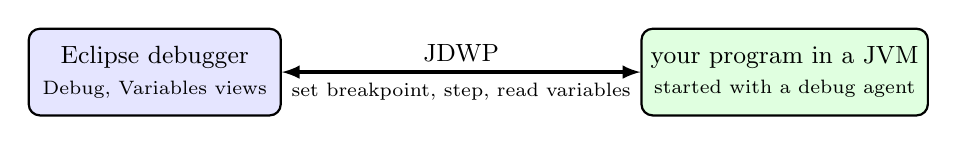
\begin{tikzpicture}[b/.style={draw, thick, rounded corners, minimum width=3.2cm, minimum height=1.1cm, align=center, font=\small}]
    \node[b, fill=blue!10] (e) at (0,0) {Eclipse debugger\\ \scriptsize Debug, Variables views};
    \node[b, fill=green!12] (j) at (8,0) {your program in a JVM\\ \scriptsize started with a debug agent};
    \draw[latex-latex, very thick] (e) -- node[above, font=\small] {JDWP} node[below, font=\scriptsize] {set breakpoint, step, read variables} (j);
  \end{tikzpicture}
  \end{center}
  \begin{itemize}\small
    \item \textbf{JDWP}, the Java Debug Wire Protocol, is a standard: Eclipse, IntelliJ, VS Code and the command-line \texttt{jdb} use it.
    \item So you can debug a program running on another machine, too (\emph{remote debugging}).
    \item The class files need debug information (line numbers, variable names); Eclipse adds it by default.
  \end{itemize}
\end{frame}
% ~~~~~~~~~~~~~~~~~~~~~~~~~~~~~~~~~~~~~~ A frm

% ~~~~~~~~~~~~~~~~~~~~~~~~~~~~~~~~~~~~~~ V
\hSection[Editing]{Help While Editing}
% ~~~~~~~~~~~~~~~~~~~~~~~~~~~~~~~~~~~~~~ A




% ~~~~~~~~~~~~~~~~~~~~~~~~~~~~~~~~~~~~~~ V frm
\begin{frame}[t,fragile] \frametitle{The editor works with you}
  \begin{center}\small
  \begin{tabular}{llll}
    \toprule
    \textbf{feature}  & \textbf{what it does}                                    & \win                 & \mac \\
    \midrule
    Content Assist    & complete names; show methods after \texttt{.}             & \keys{Ctrl+Space}    & \keys{Ctrl+Space} \\
    Quick Fix         & offer fixes for the error under the cursor                & \keys{Ctrl+1}        & \keys{\cmd+1} \\
    Templates         & \texttt{sysout}, \texttt{main}, \texttt{for} + Content Assist & \keys{Ctrl+Space} & \keys{Ctrl+Space} \\
    Format            & indent and space the code                                 & \keys{Ctrl+\shift+F} & \keys{\cmd+\shift+F} \\
    Organize Imports  & add missing, remove unused imports                        & \keys{Ctrl+\shift+O} & \keys{\cmd+\shift+O} \\
    Open Declaration  & jump to where a name is defined                           & \keys{F3}            & \keys{F3} \\
    Key Assist        & list all shortcuts                                        & \keys{Ctrl+\shift+L} & \keys{\cmd+\shift+L} \\
    \bottomrule
  \end{tabular}
  \end{center}
\end{frame}
% ~~~~~~~~~~~~~~~~~~~~~~~~~~~~~~~~~~~~~~ A frm




% ~~~~~~~~~~~~~~~~~~~~~~~~~~~~~~~~~~~~~~ V frm
\begin{frame}[t,fragile] \frametitle{Refactoring: change structure, keep behavior}
  \begin{columns}[T]
    \begin{column}{0.5\textwidth}
      \begin{center}\footnotesize
      \begin{tabular}{@{}lll@{}}
        \toprule
        \textbf{refactoring} & \win                 & \mac \\
        \midrule
        Rename               & \keys{Alt+\shift+R}  & \keys{Option+\cmd+R} \\
        Extract Method       & \keys{Alt+\shift+M}  & \keys{Option+\cmd+M} \\
        Extract Local Var.   & \keys{Alt+\shift+L}  & \keys{Option+\cmd+L} \\
        Inline               & \keys{Alt+\shift+I}  & \keys{Option+\cmd+I} \\
        \bottomrule
      \end{tabular}
      \end{center}
    \end{column}
    \begin{column}{0.46\textwidth}
      \begin{itemize}\small
        \item Rename a method: Eclipse changes the declaration \textbf{and every call}, in all files, but not
              an unrelated method or a word in a comment with the same name.
        \item Search-and-replace cannot do this: it does not know what a name \emph{means}.
        \item All refactorings: \menu{Refactor} menu; preview before applying.
      \end{itemize}
    \end{column}
  \end{columns}
\end{frame}
% ~~~~~~~~~~~~~~~~~~~~~~~~~~~~~~~~~~~~~~ A frm

% ~~~~~~~~~~~~~~~~~~~~~~~~~~~~~~~~~~~~~~ V
\hSection[Ecosystem]{Plug-ins and Tools}
% ~~~~~~~~~~~~~~~~~~~~~~~~~~~~~~~~~~~~~~ A




% ~~~~~~~~~~~~~~~~~~~~~~~~~~~~~~~~~~~~~~ V frm
\begin{frame}[t,fragile] \frametitle{Everything is a plug-in}
  \begin{columns}[T]
    \begin{column}{0.48\textwidth}
      \begin{center}
      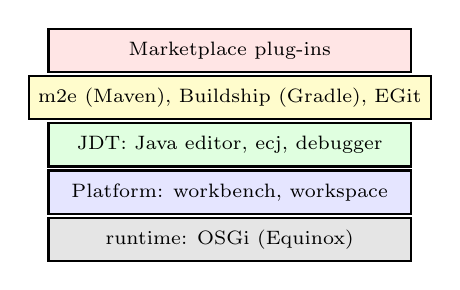
\begin{tikzpicture}[l/.style={draw, thick, minimum width=4.6cm, minimum height=0.55cm, font=\scriptsize}]
        \node[l, fill=gray!20]   at (0,0)    {runtime: OSGi (Equinox)};
        \node[l, fill=blue!10]   at (0,0.6)  {Platform: workbench, workspace};
        \node[l, fill=green!12]  at (0,1.2)  {JDT: Java editor, ecj, debugger};
        \node[l, fill=yellow!20] at (0,1.8)  {m2e (Maven), Buildship (Gradle), EGit};
        \node[l, fill=red!10]    at (0,2.4)  {Marketplace plug-ins};
      \end{tikzpicture}
      \end{center}
    \end{column}
    \begin{column}{0.48\textwidth}
      \begin{itemize}\small
        \item Eclipse is a small core plus many \textbf{plug-ins}; Java support itself is a set of plug-ins (JDT).
        \item The Java package already has Maven, Gradle and Git support.
        \item More: \menu{Help > Eclipse Marketplace\dots} \hRemark{Install only what you trust: a plug-in runs with your rights.}
      \end{itemize}
    \end{column}
  \end{columns}
\end{frame}
% ~~~~~~~~~~~~~~~~~~~~~~~~~~~~~~~~~~~~~~ A frm

% ~~~~~~~~~~~~~~~~~~~~~~~~~~~~~~~~~~~~~~ V
\hSection[Summary]{Summary}
% ~~~~~~~~~~~~~~~~~~~~~~~~~~~~~~~~~~~~~~ A




% ~~~~~~~~~~~~~~~~~~~~~~~~~~~~~~~~~~~~~~ V frm
\begin{frame}[t,fragile] \frametitle{Big ideas}
  \begin{itemize}
    \item A \textbf{workspace} holds \textbf{projects}; a Java project keeps sources in \texttt{src/}, classes in \texttt{bin/}.
    \item The \textbf{workbench} shows editors and views; a \textbf{perspective} arranges them for a job.
    \item Eclipse compiles with its own compiler \texttt{ecj} \textbf{on every save}; problems appear as markers at once.
    \item \textbf{Launch configurations} remember how to run a program; the \textbf{debugger} stops it at breakpoints (JDWP).
    \item Content Assist, Quick Fix and Refactoring work because the IDE understands the code.
    \item Eclipse is a platform of plug-ins: JDT, m2e, Buildship, EGit and many more.
  \end{itemize}
\end{frame}
% ~~~~~~~~~~~~~~~~~~~~~~~~~~~~~~~~~~~~~~ A frm




% ~~~~~~~~~~~~~~~~~~~~~~~~~~~~~~~~~~~~~~ V frm
\begin{frame}[t,fragile] \frametitle{Questions to think about}
  \begin{enumerate}\small
    \item Why can Eclipse show an error before you run the program, but not a wrong result?
    \item What is the difference between a workspace and a project? Can two workspaces share a project folder?
    \item Rename a method called \texttt{size} with search-and-replace and with \menu{Refactor > Rename}: what can go wrong with the first?
    \item Why does a debugger need the line numbers and variable names inside the class files?
    \item Find three views that are not in the Java perspective and say what they show.
  \end{enumerate}
\end{frame}
% ~~~~~~~~~~~~~~~~~~~~~~~~~~~~~~~~~~~~~~ A frm




% ~~~~~~~~~~~~~~~~~~~~~~~~~~~~~~~~~~~~~~ V frm
\begin{frame}[t,fragile]
	\begin{center}
		\vspace{4cm}
		\hRemark{\Huge Questions?}
	\end{center}
\end{frame}
% ~~~~~~~~~~~~~~~~~~~~~~~~~~~~~~~~~~~~~~ A frm



\end{document}
